\documentclass{beamer}
\usepackage{sansmathaccent}
\pdfmapfile{+sansmathaccent.map}
\usepackage{comment}
\usepackage{physics}
\usetheme{Madrid}

\usepackage[utf8]{inputenc}
\usepackage{graphicx}

\title[Rutherford Scattering]{Rutherford Scattering Detection through Gold Foil}
\author{Henry Shackleton}

\begin{document}

\titlepage

\section{Introduction and Theory}

\begin{frame}
  \frametitle{Plum Pudding and Rutherford Model}
  \begin{columns}
    \begin{column}{0.5\textwidth}
      \begin{center}
      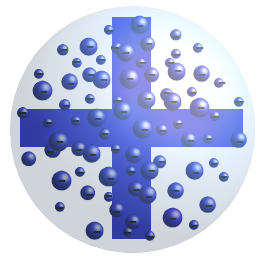
\includegraphics[width=0.5\textwidth]{plum}
      \\
      \textbf{Plum Pudding Model}
      \begin{itemize}
        \pause
        \item Small electrons in a "soup" of positive charge
          \pause
        \item Produces small-angle scattering that dies off exponentially
      \end{itemize}
    \end{center}
    \end{column}
    \begin{column}{0.5\textwidth}
      \begin{center}
      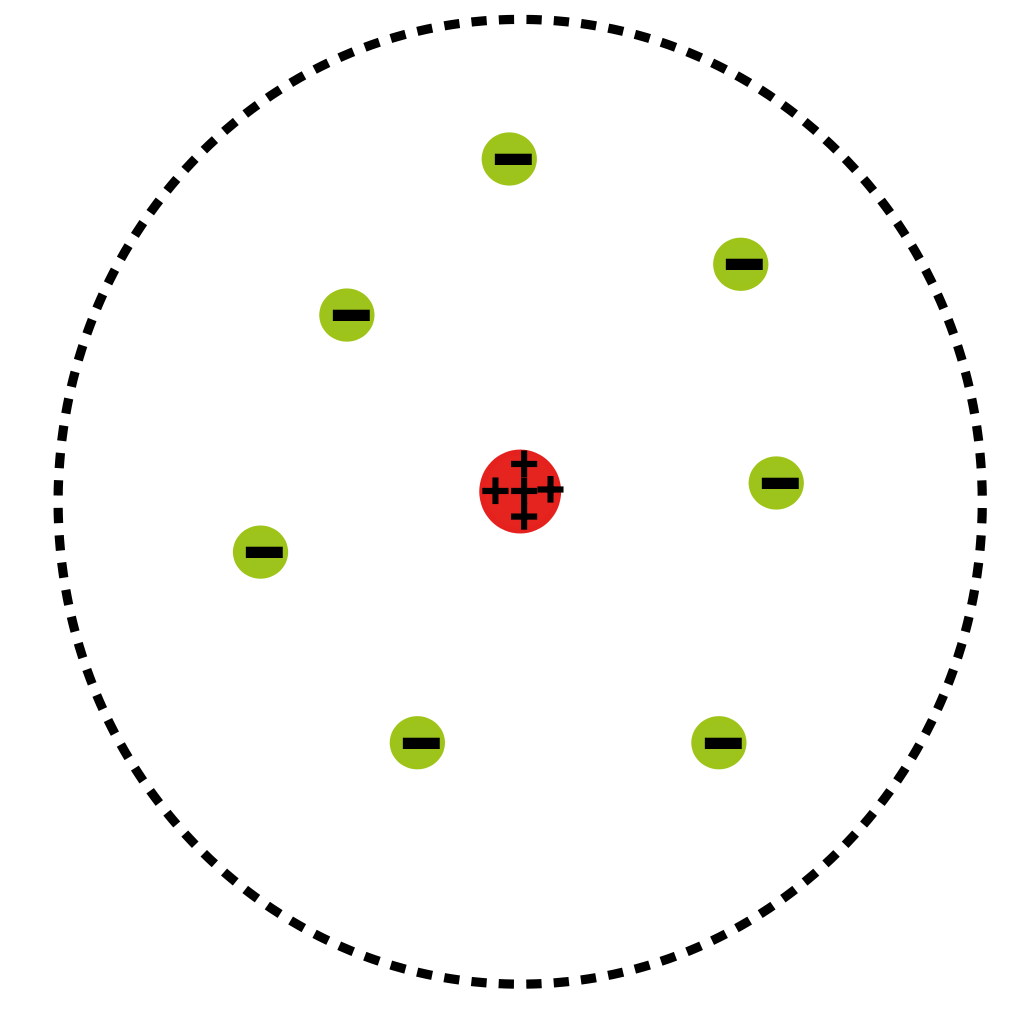
\includegraphics[width=0.44\textwidth]{rutherford.png}
      \\
      \textbf{Rutherford Model}
      \begin{itemize}
        \pause
      \item Electrons orbit around a concentrated positive charge
        \pause
      \item Allows for large scattering angles
    \end{itemize}
  \end{center}
  \end{column}
\end{columns}
\end{frame}


\begin{frame}
  \frametitle{Rutherford Scattering Derives from Coulumb Interactions}
  \begin{equation*}
    \dv{\sigma}{\Omega} = \left( \frac{Z Z' e^2}{4E}\right)^2 \frac{1}{\sin^4 (\theta/2)}
  \end{equation*}

  \begin{itemize}
    \item Differential cross section describes probability of scattering at angle $\theta$.
    \item Translation to observable trends requires consideration of flux, area density, etc., but does not affect $\theta$-dependence.
    \item Evaluating $\theta$-dependence 
  \end{itemize}
\end{frame}

\begin{frame}
  \frametitle{Apparatus allows for scattering detection at various angles}
  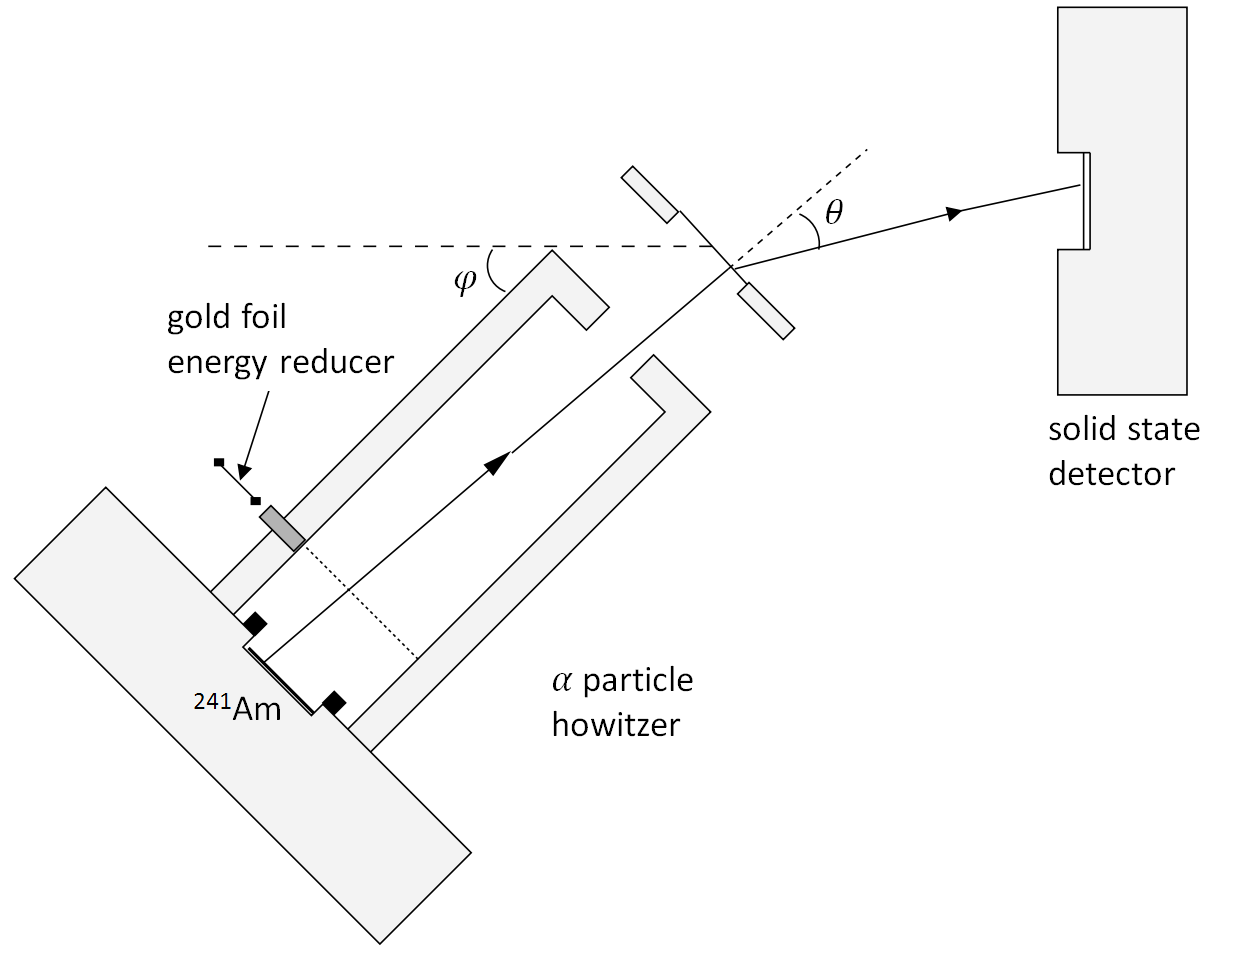
\includegraphics[width=0.8\textwidth]{apparatus}
\end{frame}




\end{document}
